Um sistema de pêndulo invertido consiste em uma haste suspensa verticalmente sobre um carro motorizado, como mostrado na \autoref{fig:Ogata2010_inverted_pendulum_diagram_complete}-a. O objetivo do controle de atitude, que é referente ao controle de orientação angular, é manter a haste na posição vertical. O pêndulo invertido é instável de forma que ele deve cair a qualquer momento e em qualquer direção a menos que uma força de controle adequada seja aplicada. Neste exemplo, é considerado um problema apenas bidimensional, em que o pêndulo se move apenas no plano da página. A força de controle $u$ é aplicada ao carro. Assume-se que o centro de gravidade da haste do pêndulo seja seu centro geométrico. Com base nestas suposições, pode-se obter um modelo matemático do sistema \cite{Ogata2010}.

\begin{figure}[!htb]
    \centering
    \caption{Diagrama do sistema de pêndulo invertido; (a) sistema de pêndulo invertido; (b) diagrama de corpo livre}
    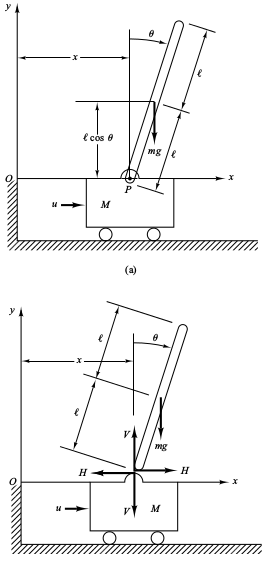
\includegraphics[width=0.55\textwidth]{./04-figuras/Ogata2010_inverted_pendulum_diagram_complete}
    \fonte{\citeonline[p.~69]{Ogata2010}}
    \label{fig:Ogata2010_inverted_pendulum_diagram_complete}
\end{figure}

Na \autoref{fig:Ogata2010_inverted_pendulum_diagram_complete}, $M$ é a massa do carro, $m$ é a massa da haste, $g$ é a força da gravidade, $x$ é o deslocamento no eixo horizontal, $l$ é metade do comprimento da haste, $\theta$ é o ângulo da haste com relação ao eixo vertical, $u$ é a força aplicada ao carro, $P$ é o ponto de rotação do pêndulo sobre o carro, $H$ é o movimento horizontal do centro de gravidade da haste do pêndulo e $V$ é o movimento vertical do centro de gravidade da haste do pêndulo. 

%\hl{Inserir diagrama de blocos do sistema}\\